% LaTeX template for Finance summaries
% Stu Alden
%----------------------------------------------------------------------------------------
\author{}  % Could include but only as small footnote

\documentclass{article}

\usepackage{amsmath}
\usepackage{tikz}
\usetikzlibrary{decorations.pathmorphing}

\title{\normalfont\ 1-A-2 Simple Discount} % The article title
\date{}  % Suppress date
\pagenumbering{gobble}

\begin{document}

    \maketitle % Print the title/author/date block

    \begin{flushleft}
        Simple Discount is also linear growth, just like Simple Interest.  They are equivalent concepts, but the terminology and labeling are different.
    \end{flushleft}

    \begin{description}
        \item\textbf{A} - amount at the beginning, or "principal" or "proceeds"
        \item\textbf{S} - amount at the end, or final amount
        \item\textbf{d} - discount rate \underline{per period}, expressed as a decimal {(\%/100)}
        \item\textbf{n} - number of periods
    \end{description}

    \begin{flushleft}
        Then we have
    \end{flushleft}

    \begin{align*}
        Amount \: of \: Interest & = I \\
        & = S \cdot d \cdot n
    \end{align*}

    \begin{flushleft}
        and
    \end{flushleft}

    \begin{align*}
        A & = S - I \\
          & = S - Sdn) \\
          & = S(1 - dn)
    \end{align*} \\

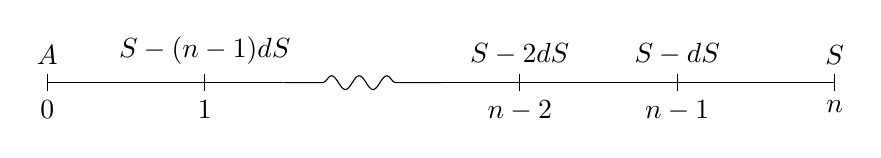
\begin{tikzpicture}
%draw horizontal line with squiggle in middle
    \draw (0,0) -- (3,0);
    \draw[decorate,decoration={snake,pre length=5mm, post length=5mm}] (3,0) -- (5,0);
    \draw (5,0) -- (10,0);

%draw vertical lines
    \foreach \x in {0,2,6,8,10}
    \draw (\x cm,3pt) -- (\x cm,-3pt);

%    {\tiny Text of first line}
%draw nodes
    \draw (0,0) node[below=3pt] {$ 0 $} node[above=3pt] {$ A $};
    \draw (2,0) node[below=3pt] {$ 1 $} node[above=3pt] {$ S-(n-1)dS $};
    \draw (6,0) node[below=3pt] {$ n-2 $} node[above=3pt] {$ S-2dS $};
    \draw (8,0) node[below=3pt] {$ n-1 $} node[above=3pt] {$ S-dS $};
    \draw (10,0) node[below=3pt] {$ n $} node[above=3pt] {$ S $};

    \newline
    \newline

\end{tikzpicture}

    \begin{center}
    {$\Leftarrow$}  {Read this way}
    \end{center}

\begin{flushleft}
        \textbf{Notes:} \\
    \end{flushleft}


    \begin{itemize}
        \item d is a percentage of the \underline{final} amount S, whereas i (simple interest) is a percentage of the \underline{beginning} amount A
        \item We can think of this as working backward and \underline{subtract} dS each period.  With simple interest, we work forward and \underline{add} Ai each period
        \item Discount rates, like interest rates, are annual, and the period is a year, unless otherwise stated
    \end{itemize}

\end{document}
